%%%%%%%%%%%%%%%%%%%%%%%%%%%%%%%%%%%%%%%%%%%%%%%%%%%%%%%%%%%%%%%%%
% Qualificacao de Doutorado / Dept Fisica, CFM, UFSC            %
% Andre@UFSC - 2015                                             %
%%%%%%%%%%%%%%%%%%%%%%%%%%%%%%%%%%%%%%%%%%%%%%%%%%%%%%%%%%%%%%%%%


%:::::::::::::::::::::::::::::::::::::::::::::::::::::::::::::::%
%                                                               %
%                       Anexo: Decomposição                     %
%                                                               %
%:::::::::::::::::::::::::::::::::::::::::::::::::::::::::::::::%

\chapter{Decomposição morfológica espectral e síntese de populações estelares
da amostra final}
\label{apendice:Decomp}


%***************************************************************%
%                                                               %
%                           K0018                               %
%                                                               %
%***************************************************************%

\section{K0018 (NGC 0155)}
\label{apendice:Decomp:K0018}

TODO Short description.

\begin{figure}
	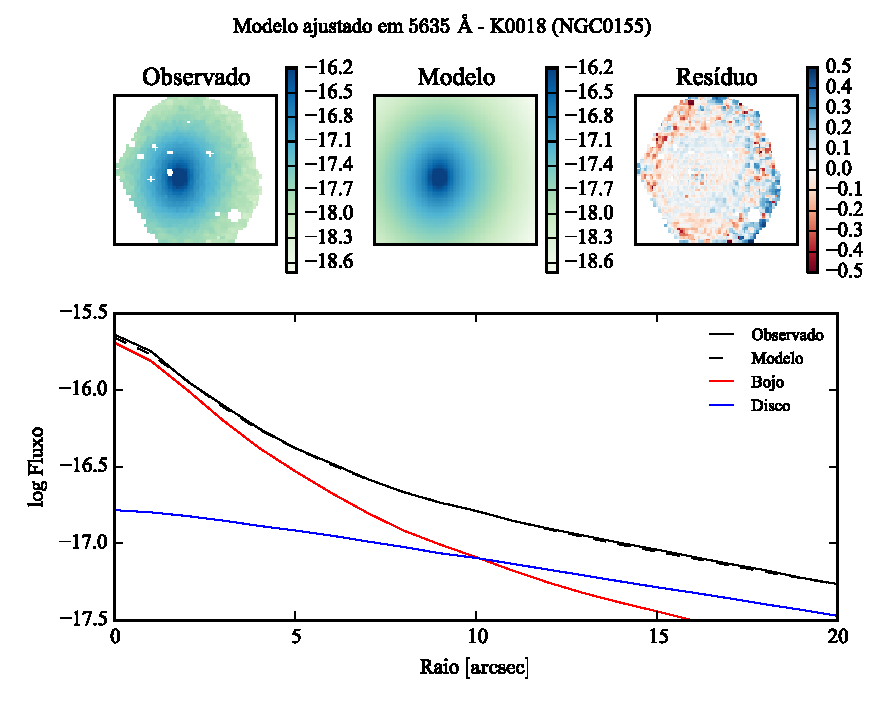
\includegraphics[page=1]{figuras-decomp/K0018_sample006a}
	\caption[Ajuste morfológico em $5635\,\angstrom$ de K0018 (NGC 0155)]
	{Acima: imagens observada, modelada e resíduo, do fluxo em $5635\,\angstrom$
	para K0018 (NGC 0155). Abaixo: perfis radiais, obtidos pela média do fluxo em
	anéis elípticos nas imagens. O fluxo observado é representado pela linha preta
	sólida. O melhor ajuste é representado pela linha preta tracejada. O bojo e o
	disco que compõe o modelo são mostrados em vermelho e azul, respectivamente.}
	\label{fig:decompRadprof:K0018}
\end{figure}

\begin{figure}
	\includegraphics[page=2]{figuras-decomp/K0018_sample006a}
	\caption[Parâmetros morfológicos em função do comprimento de onda de K0018
	(NGC 0155)]
	{Parâmetros morfológicos em função do comprimento de onda para
	K0018 (NGC 0155). Regiões em rosa representam comprimentos de onda onde a
	decomposição falhou. Regiões em cinza foram mascaradas antes de iniciar a
	decomposição. Pontos azuis indicam o primeiro passo da decomposição, em caixas
	de $100\,\angstrom$.}
	\label{fig:decompParams:K0018}
\end{figure}

\begin{figure}
	\includegraphics[page=3]{figuras-decomp/K0018_sample006a}
	\caption[Imagens em $5635\,\angstrom$ das componentes morfológicas de K0018
	(NGC 0155)]
	{Imagens em $5635\,\angstrom$ das componentes morfológicas de K0018
	(NGC 0155).}
	\label{fig:decompImages:K0018}
\end{figure}

\begin{figure}
	\includegraphics[page=4]{figuras-decomp/K0018_sample006a}
	\caption[Espectro das componentes morfológicas de K0018 (NGC 0155)]
	{Espectro das componentes morfológicas de K0018 (NGC 0155),
	observado (preto), bojo (vermelho), disco (azul) e resíduo (magenta). Acima:
	Espectro do {\em spaxel} nuclear da galáxia. Meio: Espectro em um {\em spaxel}
	a uma distância de $r_e$ do núcleo. Abaixo: Espectro integrado espacialmente.}
	\label{fig:decompSpectra:K0018}
\end{figure}

\begin{figure}
	\includegraphics[page=5]{figuras-decomp/K0018_sample006a}
	\caption[Perfis radiais para diversos comprimentos de onda de K0018 (NGC 0155)]
	{Perfis radiais para diversos comprimentos de onda de K0018 (NGC 0155).}
	\label{fig:decompRadprofSpec:K0018}
\end{figure}

%***************************************************************%
%                                                               %
%                           K0127                               %
%                                                               %
%***************************************************************%

\section{K0127 (NGC 1349)}
\label{apendice:Decomp:K0127}

TODO Short description.

\begin{figure}
	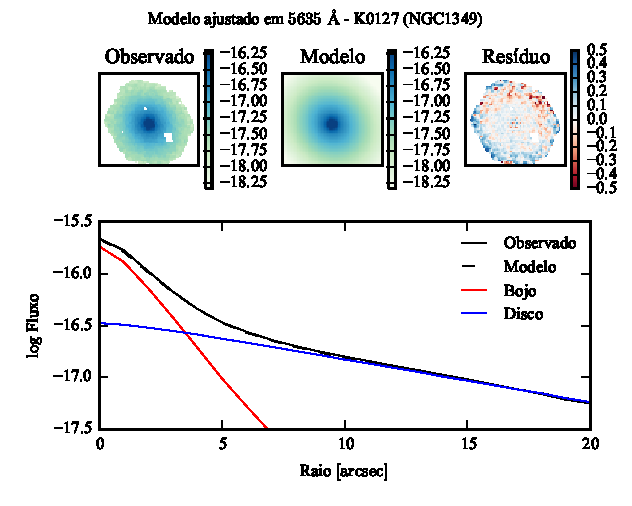
\includegraphics[page=1]{figuras-decomp/K0127_sample006a}
	\caption[Ajuste morfológico em $5635\,\angstrom$ de K0127 (NGC 1349)]
	{Acima: imagens observada, modelada e resíduo, do fluxo em $5635\,\angstrom$
	para K0127 (NGC 1349). Abaixo: perfis radiais, obtidos pela média do fluxo em
	anéis elípticos nas imagens. O fluxo observado é representado pela linha preta
	sólida. O melhor ajuste é representado pela linha preta tracejada. O bojo e o
	disco que compõe o modelo são mostrados em vermelho e azul, respectivamente.}
	\label{fig:decompRadprof:K0127}
\end{figure}

\begin{figure}
	\includegraphics[page=2]{figuras-decomp/K0127_sample006a}
	\caption[Parâmetros morfológicos em função do comprimento de onda de K0127
	(NGC 1349)]
	{Parâmetros morfológicos em função do comprimento de onda para
	K0127 (NGC 1349). Regiões em rosa representam comprimentos de onda onde a
	decomposição falhou. Regiões em cinza foram mascaradas antes de iniciar a
	decomposição. Pontos azuis indicam o primeiro passo da decomposição, em caixas
	de $100\,\angstrom$.}
	\label{fig:decompParams:K0127}
\end{figure}

\begin{figure}
	\includegraphics[page=3]{figuras-decomp/K0127_sample006a}
	\caption[Imagens em $5635\,\angstrom$ das componentes morfológicas de K0127
	(NGC 1349)]
	{Imagens em $5635\,\angstrom$ das componentes morfológicas de K0127
	(NGC 1349).}
	\label{fig:decompImages:K0127}
\end{figure}

\begin{figure}
	\includegraphics[page=4]{figuras-decomp/K0127_sample006a}
	\caption[Espectro das componentes morfológicas de K0127 (NGC 1349)]
	{Espectro das componentes morfológicas de K0127 (NGC 1349),
	observado (preto), bojo (vermelho), disco (azul) e resíduo (magenta). Acima:
	Espectro do {\em spaxel} nuclear da galáxia. Meio: Espectro em um {\em spaxel}
	a uma distância de $r_e$ do núcleo. Abaixo: Espectro integrado espacialmente.}
	\label{fig:decompSpectra:K0127}
\end{figure}

\begin{figure}
	\includegraphics[page=5]{figuras-decomp/K0127_sample006a}
	\caption[Perfis radiais para diversos comprimentos de onda de K0127 (NGC 1349)]
	{Perfis radiais para diversos comprimentos de onda de K0127 (NGC 1349).}
	\label{fig:decompRadprofSpec:K0127}
\end{figure}

%***************************************************************%
%                                                               %
%                           K0592                               %
%                                                               %
%***************************************************************%

\section{K0592 (NGC 4874)}
\label{apendice:Decomp:K0592}

TODO Short description.

\begin{figure}
	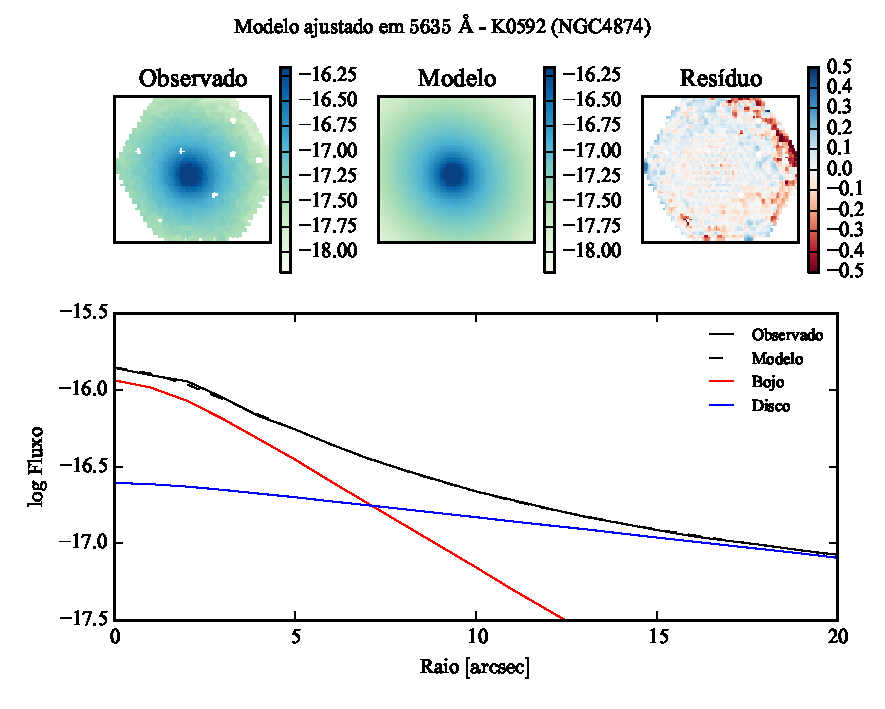
\includegraphics[page=1]{figuras-decomp/K0592_sample006a}
	\caption[Ajuste morfológico em $5635\,\angstrom$ de K0592 (NGC 4874)]
	{Acima: imagens observada, modelada e resíduo, do fluxo em $5635\,\angstrom$
	para K0592 (NGC 4874). Abaixo: perfis radiais, obtidos pela média do fluxo em
	anéis elípticos nas imagens. O fluxo observado é representado pela linha preta
	sólida. O melhor ajuste é representado pela linha preta tracejada. O bojo e o
	disco que compõe o modelo são mostrados em vermelho e azul, respectivamente.}
	\label{fig:decompRadprof:K0592}
\end{figure}

\begin{figure}
	\includegraphics[page=2]{figuras-decomp/K0592_sample006a}
	\caption[Parâmetros morfológicos em função do comprimento de onda de K0592
	(NGC 4874)]
	{Parâmetros morfológicos em função do comprimento de onda para
	K0592 (NGC 4874). Regiões em rosa representam comprimentos de onda onde a
	decomposição falhou. Regiões em cinza foram mascaradas antes de iniciar a
	decomposição. Pontos azuis indicam o primeiro passo da decomposição, em caixas
	de $100\,\angstrom$.}
	\label{fig:decompParams:K0592}
\end{figure}

\begin{figure}
	\includegraphics[page=3]{figuras-decomp/K0592_sample006a}
	\caption[Imagens em $5635\,\angstrom$ das componentes morfológicas de K0592
	(NGC 4874)]
	{Imagens em $5635\,\angstrom$ das componentes morfológicas de K0592
	(NGC 4874).}
	\label{fig:decompImages:K0592}
\end{figure}

\begin{figure}
	\includegraphics[page=4]{figuras-decomp/K0592_sample006a}
	\caption[Espectro das componentes morfológicas de K0592 (NGC 4874)]
	{Espectro das componentes morfológicas de K0592 (NGC 4874),
	observado (preto), bojo (vermelho), disco (azul) e resíduo (magenta). Acima:
	Espectro do {\em spaxel} nuclear da galáxia. Meio: Espectro em um {\em spaxel}
	a uma distância de $r_e$ do núcleo. Abaixo: Espectro integrado espacialmente.}
	\label{fig:decompSpectra:K0592}
\end{figure}

\begin{figure}
	\includegraphics[page=5]{figuras-decomp/K0592_sample006a}
	\caption[Perfis radiais para diversos comprimentos de onda de K0592 (NGC 4874)]
	{Perfis radiais para diversos comprimentos de onda de K0592 (NGC 4874).}
	\label{fig:decompRadprofSpec:K0592}
\end{figure}

%***************************************************************%
%                                                               %
%                           K0602                               %
%                                                               %
%***************************************************************%

\section{K0602 (NGC 4956)}
\label{apendice:Decomp:K0602}

TODO Short description.

\begin{figure}
	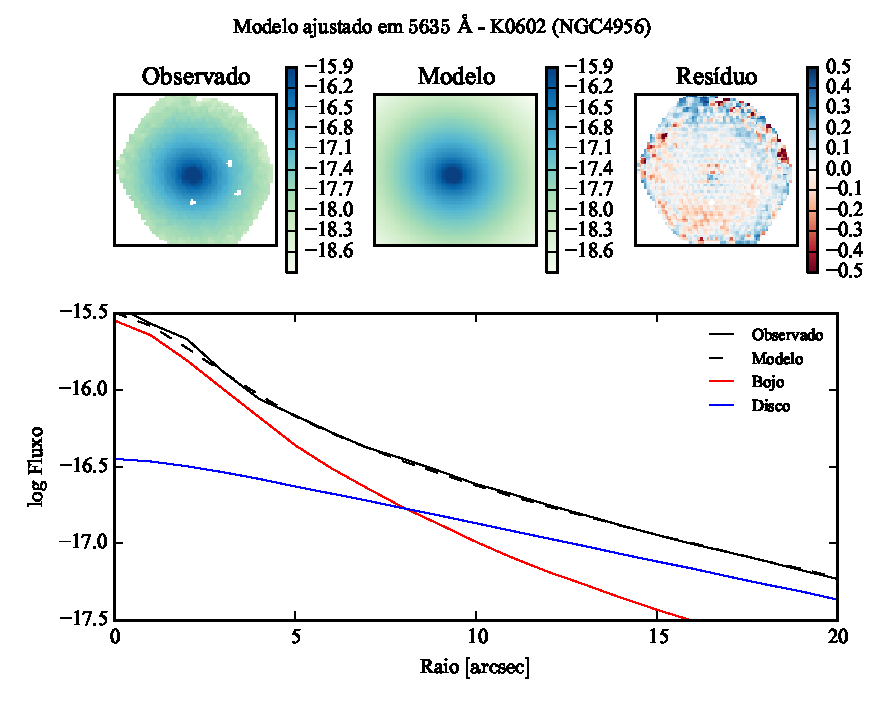
\includegraphics[page=1]{figuras-decomp/K0602_sample006a}
	\caption[Ajuste morfológico em $5635\,\angstrom$ de K0602 (NGC 4956)]
	{Acima: imagens observada, modelada e resíduo, do fluxo em $5635\,\angstrom$
	para K0602 (NGC 4956). Abaixo: perfis radiais, obtidos pela média do fluxo em
	anéis elípticos nas imagens. O fluxo observado é representado pela linha preta
	sólida. O melhor ajuste é representado pela linha preta tracejada. O bojo e o
	disco que compõe o modelo são mostrados em vermelho e azul, respectivamente.}
	\label{fig:decompRadprof:K0602}
\end{figure}

\begin{figure}
	\includegraphics[page=2]{figuras-decomp/K0602_sample006a}
	\caption[Parâmetros morfológicos em função do comprimento de onda de K0602
	(NGC 4956)]
	{Parâmetros morfológicos em função do comprimento de onda para
	K0602 (NGC 4956). Regiões em rosa representam comprimentos de onda onde a
	decomposição falhou. Regiões em cinza foram mascaradas antes de iniciar a
	decomposição. Pontos azuis indicam o primeiro passo da decomposição, em caixas
	de $100\,\angstrom$.}
	\label{fig:decompParams:K0602}
\end{figure}

\begin{figure}
	\includegraphics[page=3]{figuras-decomp/K0602_sample006a}
	\caption[Imagens em $5635\,\angstrom$ das componentes morfológicas de K0602
	(NGC 4956)]
	{Imagens em $5635\,\angstrom$ das componentes morfológicas de K0602
	(NGC 4956).}
	\label{fig:decompImages:K0602}
\end{figure}

\begin{figure}
	\includegraphics[page=4]{figuras-decomp/K0602_sample006a}
	\caption[Espectro das componentes morfológicas de K0602 (NGC 4956)]
	{Espectro das componentes morfológicas de K0602 (NGC 4956),
	observado (preto), bojo (vermelho), disco (azul) e resíduo (magenta). Acima:
	Espectro do {\em spaxel} nuclear da galáxia. Meio: Espectro em um {\em spaxel}
	a uma distância de $r_e$ do núcleo. Abaixo: Espectro integrado espacialmente.}
	\label{fig:decompSpectra:K0602}
\end{figure}

\begin{figure}
	\includegraphics[page=5]{figuras-decomp/K0602_sample006a}
	\caption[Perfis radiais para diversos comprimentos de onda de K0602 (NGC 4956)]
	{Perfis radiais para diversos comprimentos de onda de K0602 (NGC 4956).}
	\label{fig:decompRadprofSpec:K0602}
\end{figure}

%***************************************************************%
%                                                               %
%                           K0832                               %
%                                                               %
%***************************************************************%

\section{K0832 (NGC 6146)}
\label{apendice:Decomp:K0832}

TODO Short description.

\begin{figure}
	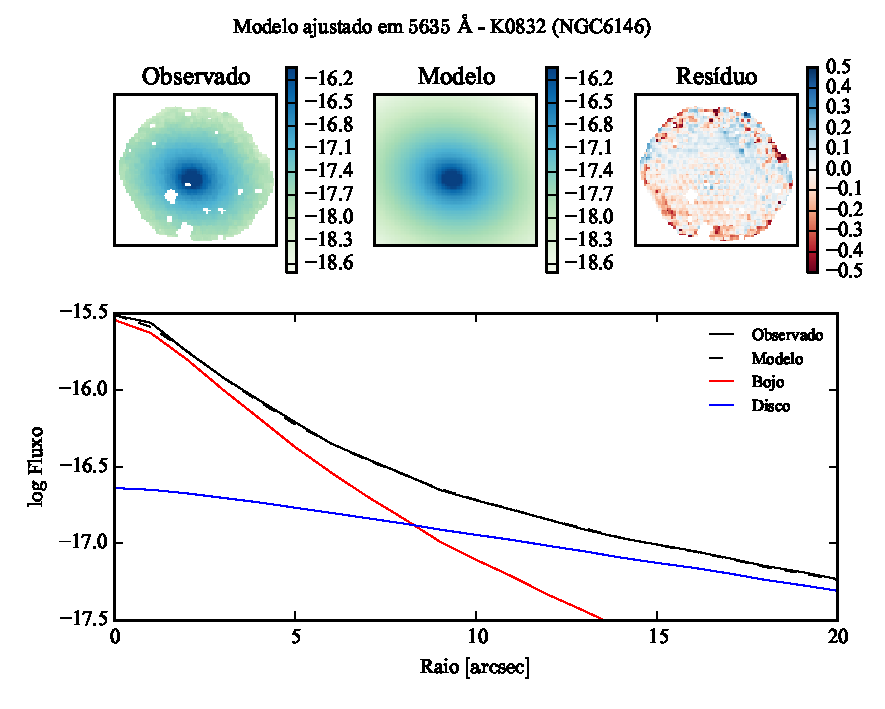
\includegraphics[page=1]{figuras-decomp/K0832_sample006a}
	\caption[Ajuste morfológico em $5635\,\angstrom$ de K0832 (NGC 6146)]
	{Acima: imagens observada, modelada e resíduo, do fluxo em $5635\,\angstrom$
	para K0832 (NGC 6146). Abaixo: perfis radiais, obtidos pela média do fluxo em
	anéis elípticos nas imagens. O fluxo observado é representado pela linha preta
	sólida. O melhor ajuste é representado pela linha preta tracejada. O bojo e o
	disco que compõe o modelo são mostrados em vermelho e azul, respectivamente.}
	\label{fig:decompRadprof:K0832}
\end{figure}

\begin{figure}
	\includegraphics[page=2]{figuras-decomp/K0832_sample006a}
	\caption[Parâmetros morfológicos em função do comprimento de onda de K0832
	(NGC 6146)]
	{Parâmetros morfológicos em função do comprimento de onda para
	K0832 (NGC 6146). Regiões em rosa representam comprimentos de onda onde a
	decomposição falhou. Regiões em cinza foram mascaradas antes de iniciar a
	decomposição. Pontos azuis indicam o primeiro passo da decomposição, em caixas
	de $100\,\angstrom$.}
	\label{fig:decompParams:K0832}
\end{figure}

\begin{figure}
	\includegraphics[page=3]{figuras-decomp/K0832_sample006a}
	\caption[Imagens em $5635\,\angstrom$ das componentes morfológicas de K0832
	(NGC 6146)]
	{Imagens em $5635\,\angstrom$ das componentes morfológicas de K0832
	(NGC 6146).}
	\label{fig:decompImages:K0832}
\end{figure}

\begin{figure}
	\includegraphics[page=4]{figuras-decomp/K0832_sample006a}
	\caption[Espectro das componentes morfológicas de K0832 (NGC 6146)]
	{Espectro das componentes morfológicas de K0832 (NGC 6146),
	observado (preto), bojo (vermelho), disco (azul) e resíduo (magenta). Acima:
	Espectro do {\em spaxel} nuclear da galáxia. Meio: Espectro em um {\em spaxel}
	a uma distância de $r_e$ do núcleo. Abaixo: Espectro integrado espacialmente.}
	\label{fig:decompSpectra:K0832}
\end{figure}

\begin{figure}
	\includegraphics[page=5]{figuras-decomp/K0832_sample006a}
	\caption[Perfis radiais para diversos comprimentos de onda de K0832 (NGC 6146)]
	{Perfis radiais para diversos comprimentos de onda de K0832 (NGC 6146).}
	\label{fig:decompRadprofSpec:K0832}
\end{figure}

%***************************************************************%
%                                                               %
%                           K0846                               %
%                                                               %
%***************************************************************%

\section{K0846 (UGC 10695)}
\label{apendice:Decomp:K0846}

TODO Short description.

\begin{figure}
	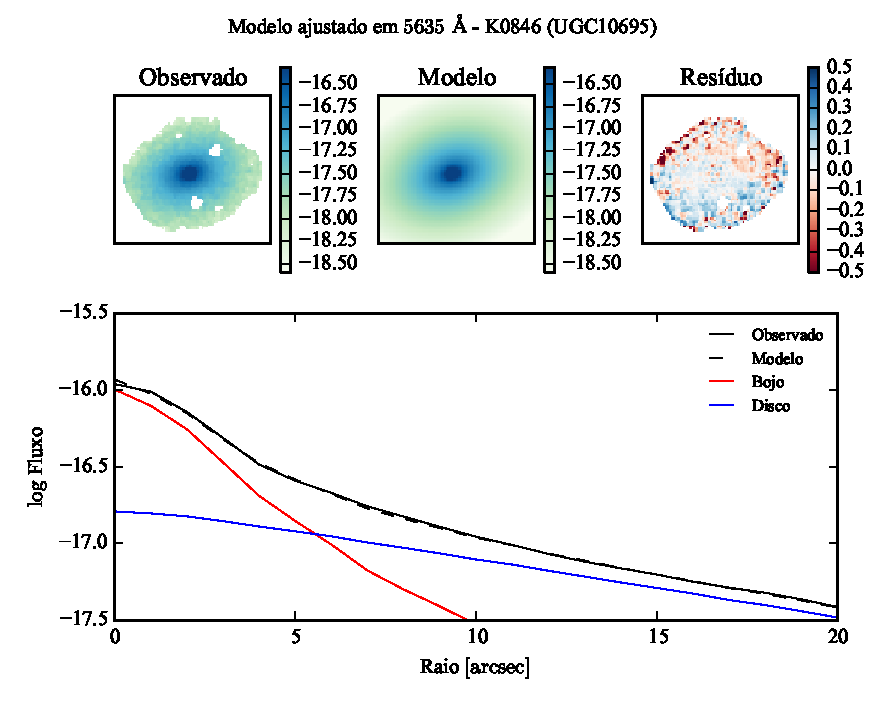
\includegraphics[page=1]{figuras-decomp/K0846_sample006a}
	\caption[Ajuste morfológico em $5635\,\angstrom$ de K0846 (UGC 10695)]
	{Acima: imagens observada, modelada e resíduo, do fluxo em $5635\,\angstrom$
	para K0846 (UGC 10695). Abaixo: perfis radiais, obtidos pela média do fluxo em
	anéis elípticos nas imagens. O fluxo observado é representado pela linha preta
	sólida. O melhor ajuste é representado pela linha preta tracejada. O bojo e o
	disco que compõe o modelo são mostrados em vermelho e azul, respectivamente.}
	\label{fig:decompRadprof:K0846}
\end{figure}

\begin{figure}
	\includegraphics[page=2]{figuras-decomp/K0846_sample006a}
	\caption[Parâmetros morfológicos em função do comprimento de onda de K0846
	(UGC 10695)]
	{Parâmetros morfológicos em função do comprimento de onda para
	K0846 (UGC 10695). Regiões em rosa representam comprimentos de onda onde a
	decomposição falhou. Regiões em cinza foram mascaradas antes de iniciar a
	decomposição. Pontos azuis indicam o primeiro passo da decomposição, em caixas
	de $100\,\angstrom$.}
	\label{fig:decompParams:K0846}
\end{figure}

\begin{figure}
	\includegraphics[page=3]{figuras-decomp/K0846_sample006a}
	\caption[Imagens em $5635\,\angstrom$ das componentes morfológicas de K0846
	(UGC 10695)]
	{Imagens em $5635\,\angstrom$ das componentes morfológicas de K0846
	(UGC 10695).}
	\label{fig:decompImages:K0846}
\end{figure}

\begin{figure}
	\includegraphics[page=4]{figuras-decomp/K0846_sample006a}
	\caption[Espectro das componentes morfológicas de K0846 (UGC 10695)]
	{Espectro das componentes morfológicas de K0846 (UGC 10695),
	observado (preto), bojo (vermelho), disco (azul) e resíduo (magenta). Acima:
	Espectro do {\em spaxel} nuclear da galáxia. Meio: Espectro em um {\em spaxel}
	a uma distância de $r_e$ do núcleo. Abaixo: Espectro integrado espacialmente.}
	\label{fig:decompSpectra:K0846}
\end{figure}

\begin{figure}
	\includegraphics[page=5]{figuras-decomp/K0846_sample006a}
	\caption[Perfis radiais para diversos comprimentos de onda de K0846 (UGC 10695)]
	{Perfis radiais para diversos comprimentos de onda de K0846 (UGC 10695).}
	\label{fig:decompRadprofSpec:K0846}
\end{figure}

%***************************************************************%
%                                                               %
%                           K0851                               %
%                                                               %
%***************************************************************%

\section{K0851 (NGC 6338)}
\label{apendice:Decomp:K0851}

TODO Short description.

\begin{figure}
	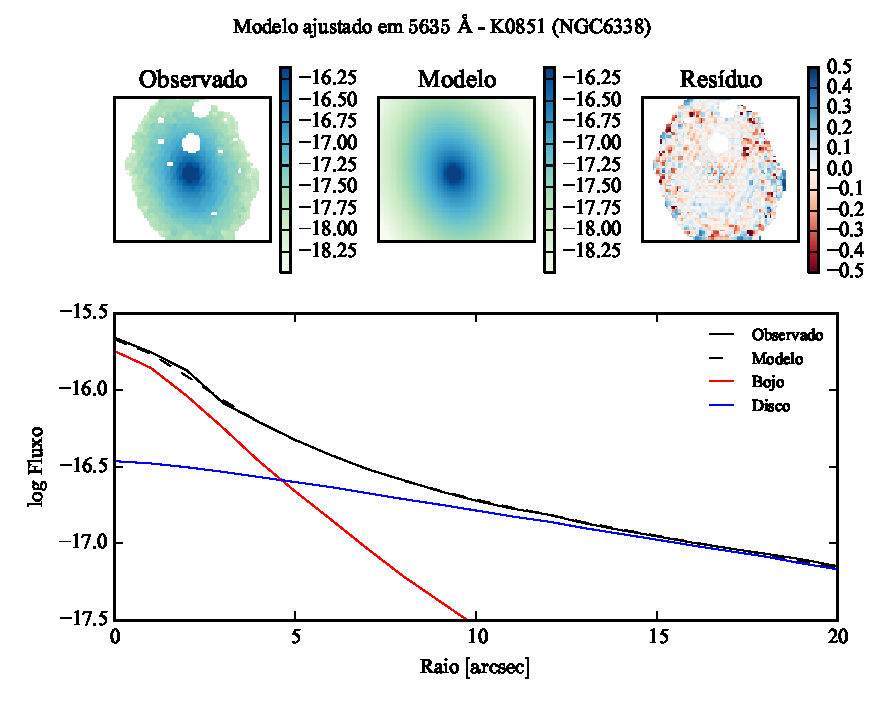
\includegraphics[page=1]{figuras-decomp/K0851_sample006a}
	\caption[Ajuste morfológico em $5635\,\angstrom$ de K0851 (NGC 6338)]
	{Acima: imagens observada, modelada e resíduo, do fluxo em $5635\,\angstrom$
	para K0851 (NGC 6338). Abaixo: perfis radiais, obtidos pela média do fluxo em
	anéis elípticos nas imagens. O fluxo observado é representado pela linha preta
	sólida. O melhor ajuste é representado pela linha preta tracejada. O bojo e o
	disco que compõe o modelo são mostrados em vermelho e azul, respectivamente.}
	\label{fig:decompRadprof:K0851}
\end{figure}

\begin{figure}
	\includegraphics[page=2]{figuras-decomp/K0851_sample006a}
	\caption[Parâmetros morfológicos em função do comprimento de onda de K0851
	(NGC 6338)]
	{Parâmetros morfológicos em função do comprimento de onda para
	K0851 (NGC 6338). Regiões em rosa representam comprimentos de onda onde a
	decomposição falhou. Regiões em cinza foram mascaradas antes de iniciar a
	decomposição. Pontos azuis indicam o primeiro passo da decomposição, em caixas
	de $100\,\angstrom$.}
	\label{fig:decompParams:K0851}
\end{figure}

\begin{figure}
	\includegraphics[page=3]{figuras-decomp/K0851_sample006a}
	\caption[Imagens em $5635\,\angstrom$ das componentes morfológicas de K0851
	(NGC 6338)]
	{Imagens em $5635\,\angstrom$ das componentes morfológicas de K0851
	(NGC 6338).}
	\label{fig:decompImages:K0851}
\end{figure}

\begin{figure}
	\includegraphics[page=4]{figuras-decomp/K0851_sample006a}
	\caption[Espectro das componentes morfológicas de K0851 (NGC 6338)]
	{Espectro das componentes morfológicas de K0851 (NGC 6338),
	observado (preto), bojo (vermelho), disco (azul) e resíduo (magenta). Acima:
	Espectro do {\em spaxel} nuclear da galáxia. Meio: Espectro em um {\em spaxel}
	a uma distância de $r_e$ do núcleo. Abaixo: Espectro integrado espacialmente.}
	\label{fig:decompSpectra:K0851}
\end{figure}

\begin{figure}
	\includegraphics[page=5]{figuras-decomp/K0851_sample006a}
	\caption[Perfis radiais para diversos comprimentos de onda de K0851 (NGC 6338)]
	{Perfis radiais para diversos comprimentos de onda de K0851 (NGC 6338).}
	\label{fig:decompRadprofSpec:K0851}
\end{figure}

%***************************************************************%
%                                                               %
%                           K0858                               %
%                                                               %
%***************************************************************%

\section{K0858 (UGC 10905)}
\label{apendice:Decomp:K00858}

TODO Short description.

\begin{figure}
	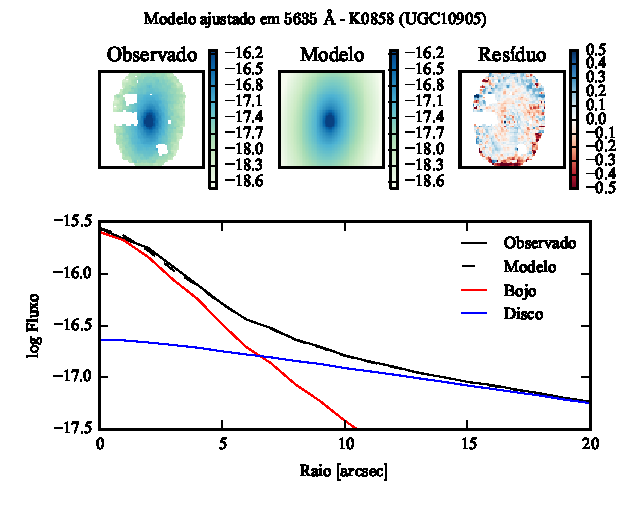
\includegraphics[page=1]{figuras-decomp/K0858_sample006a}
	\caption[Ajuste morfológico em $5635\,\angstrom$ de K0858 (UGC 10905)]
	{Acima: imagens observada, modelada e resíduo, do fluxo em $5635\,\angstrom$
	para K0858 (UGC 10905). Abaixo: perfis radiais, obtidos pela média do fluxo em
	anéis elípticos nas imagens. O fluxo observado é representado pela linha preta
	sólida. O melhor ajuste é representado pela linha preta tracejada. O bojo e o
	disco que compõe o modelo são mostrados em vermelho e azul, respectivamente.}
	\label{fig:decompRadprof:K0858}
\end{figure}

\begin{figure}
	\includegraphics[page=2]{figuras-decomp/K0858_sample006a}
	\caption[Parâmetros morfológicos em função do comprimento de onda de K0858
	(UGC 10905)]
	{Parâmetros morfológicos em função do comprimento de onda para
	K0858 (UGC 10905). Regiões em rosa representam comprimentos de onda onde a
	decomposição falhou. Regiões em cinza foram mascaradas antes de iniciar a
	decomposição. Pontos azuis indicam o primeiro passo da decomposição, em caixas
	de $100\,\angstrom$.}
	\label{fig:decompParams:K0858}
\end{figure}

\begin{figure}
	\includegraphics[page=3]{figuras-decomp/K0858_sample006a}
	\caption[Imagens em $5635\,\angstrom$ das componentes morfológicas de K0858
	(UGC 10905)]
	{Imagens em $5635\,\angstrom$ das componentes morfológicas de K0858
	(UGC 10905).}
	\label{fig:decompImages:K0858}
\end{figure}

\begin{figure}
	\includegraphics[page=4]{figuras-decomp/K0858_sample006a}
	\caption[Espectro das componentes morfológicas de K0858 (UGC 10905)]
	{Espectro das componentes morfológicas de K0858 (UGC 10905),
	observado (preto), bojo (vermelho), disco (azul) e resíduo (magenta). Acima:
	Espectro do {\em spaxel} nuclear da galáxia. Meio: Espectro em um {\em spaxel}
	a uma distância de $r_e$ do núcleo. Abaixo: Espectro integrado espacialmente.}
	\label{fig:decompSpectra:K0858}
\end{figure}

\begin{figure}
	\includegraphics[page=5]{figuras-decomp/K0858_sample006a}
	\caption[Perfis radiais para diversos comprimentos de onda de K0858 (UGC 10905)]
	{Perfis radiais para diversos comprimentos de onda de K0858 (UGC 10905).}
	\label{fig:decompRadprofSpec:K0858}
\end{figure}

%***************************************************************%
%                                                               %
%                           K0912                               %
%                                                               %
%***************************************************************%

\section{K0912 (NGC 7623)}
\label{apendice:Decomp:K0912}

TODO Short description.

\begin{figure}
	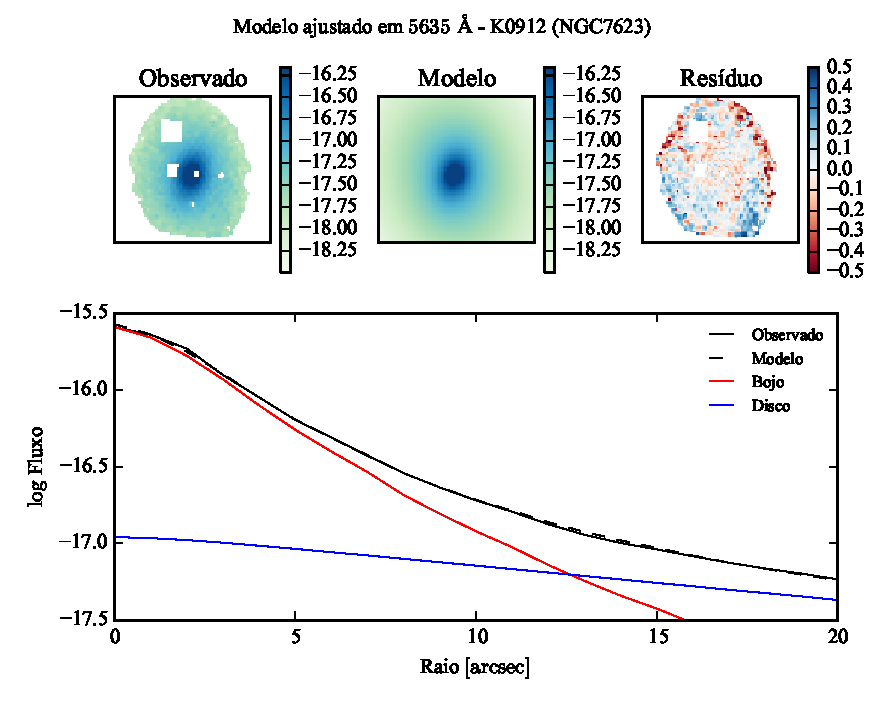
\includegraphics[page=1]{figuras-decomp/K0912_sample006a}
	\caption[Ajuste morfológico em $5635\,\angstrom$ de K0912 (NGC 7623)]
	{Acima: imagens observada, modelada e resíduo, do fluxo em $5635\,\angstrom$
	para K0912 (NGC 7623). Abaixo: perfis radiais, obtidos pela média do fluxo em
	anéis elípticos nas imagens. O fluxo observado é representado pela linha preta
	sólida. O melhor ajuste é representado pela linha preta tracejada. O bojo e o
	disco que compõe o modelo são mostrados em vermelho e azul, respectivamente.}
	\label{fig:decompRadprof:K0912}
\end{figure}

\begin{figure}
	\includegraphics[page=2]{figuras-decomp/K0912_sample006a}
	\caption[Parâmetros morfológicos em função do comprimento de onda de K0912
	(NGC 7623)]
	{Parâmetros morfológicos em função do comprimento de onda para
	K0912 (NGC 7623). Regiões em rosa representam comprimentos de onda onde a
	decomposição falhou. Regiões em cinza foram mascaradas antes de iniciar a
	decomposição. Pontos azuis indicam o primeiro passo da decomposição, em caixas
	de $100\,\angstrom$.}
	\label{fig:decompParams:K0912}
\end{figure}

\begin{figure}
	\includegraphics[page=3]{figuras-decomp/K0912_sample006a}
	\caption[Imagens em $5635\,\angstrom$ das componentes morfológicas de K0912
	(NGC 7623)]
	{Imagens em $5635\,\angstrom$ das componentes morfológicas de K0912
	(NGC 7623).}
	\label{fig:decompImages:K0912}
\end{figure}

\begin{figure}
	\includegraphics[page=4]{figuras-decomp/K0912_sample006a}
	\caption[Espectro das componentes morfológicas de K0912 (NGC 7623)]
	{Espectro das componentes morfológicas de K0912 (NGC 7623),
	observado (preto), bojo (vermelho), disco (azul) e resíduo (magenta). Acima:
	Espectro do {\em spaxel} nuclear da galáxia. Meio: Espectro em um {\em spaxel}
	a uma distância de $r_e$ do núcleo. Abaixo: Espectro integrado espacialmente.}
	\label{fig:decompSpectra:K0912}
\end{figure}

\begin{figure}
	\includegraphics[page=5]{figuras-decomp/K0912_sample006a}
	\caption[Perfis radiais para diversos comprimentos de onda de K0912 (NGC 7623)]
	{Perfis radiais para diversos comprimentos de onda de K0912 (NGC 7623).}
	\label{fig:decompRadprofSpec:K0912}
\end{figure}

% End of this chapter
